\documentclass[conference]{IEEEtran}
\IEEEoverridecommandlockouts

% Standard IEEE packages
\usepackage{cite}
\usepackage{amsmath,amssymb,amsfonts}
\usepackage{algorithmic}
\usepackage{graphicx}
\usepackage{textcomp}
\usepackage{xcolor}
\usepackage{booktabs}
\usepackage{multirow}
\usepackage{url}
\usepackage{placeins}
\usepackage[hidelinks]{hyperref}

\def\BibTeX{{\rm B\kern-.05em{\sc i\kern-.025em b}\kern-.08em
    T\kern-.1667em\lower.7ex\hbox{E}\kern-.125emX}}

\begin{document}

\title{RiceGuard: Lesion-Grounded Multi-Task Deep Learning for Rice Leaf Disease Classification, Localization, and Quantitative Explainability}

\author{
\begin{tabular}[t]{c}
\textbf{Varad Hiraman Parate, Dhruv A. Gholap, Hrushikesh Suryawanshi, and Arnav Kulkarni} \\
Department of Information Technology \\
Vishwakarma Institute of Information Technology \\
Pune, Maharashtra, India \\
\texttt{\{varad.22311382, dhruv.22311579, hrushikesh.22310354, arnav.22310597\}@viit.ac.in} \\[2.2ex]
\textbf{Dr. Shalini Wankhade} \\
Department of Information Technology \\
Vishwakarma Institute of Technology \\
Pune, Maharashtra, India \\
\texttt{shalini.wankhade@vit.edu}
\end{tabular}
}

\maketitle

\begin{abstract}
Automated rice leaf pathology classification using deep convolutional neural networks has achieved strong benchmark performance. However, standard classification models predict categorical disease labels without explicit spatial evidence identifying specific lesion regions, frequently learning spurious background and border correlations. In this work, we present RiceGuard, an empirical study evaluating whether weak spatial supervision using bounding-box lesion annotations can provide spatial lesion localization capability while assessing its impact on disease classification and explainability. Built upon an EfficientNet-B0 backbone, RiceGuard jointly optimizes six-class disease classification and $7\times 7$ grid-based lesion localization. A controlled refinement procedure (Phase 3B) addresses foreground-background objectness imbalance via capped positive class weighting ($\text{pos\_weight}=10.00$) and validation-only confidence calibration ($\tau=0.60$, Top-$K=3$). Evaluated on the RiceLeafDiseaseBD benchmark, the Phase 2B classification baseline achieves 90.12\% accuracy and 0.8891 Macro F1, while the Phase 3B multi-task model achieves 88.96\% accuracy, 0.8751 Macro F1, a Localization F1 of 0.0905, and a Mean Matched IoU of 0.6423. Calibration reduces the healthy leaf false positive rate from 21.52\% to 10.97\% and decreases border attention from 18.5\% to 9.2\%. Quantitative Grad-CAM validation against independent RiceSeg5932 segmentation masks demonstrates a slight directional gain in Pointing Game accuracy on mutually correctly classified samples (38.21\% vs. 36.79\%), while all-sample continuous alignment metrics reflect cross-domain distribution shifts. The findings demonstrate that bounding-box multi-task learning successfully imparts spatial localization capability and suppresses background shortcut reliance, accompanied by a measurable, limited classification trade-off.
\end{abstract}

\begin{IEEEkeywords}
Rice leaf disease classification, deep learning, EfficientNet, multi-task learning, lesion localization, explainable artificial intelligence, Grad-CAM, agricultural AI.
\end{IEEEkeywords}


\section{Introduction}
\label{sec:introduction}

\IEEEPARstart{R}{ice} (\textit{Oryza sativa}) is a primary nutritional staple for over half of the global population. Agricultural yields are severely threatened by foliar diseases, notably Rice Blast, Brown Spot, Leaf Smut, Tungro, and Sheath Blight, which can cause substantial annual harvest losses when left unmanaged \cite{ref2, ref15}. Automated computer vision systems leveraging deep learning and convolutional neural networks (CNNs) have emerged as essential tools for scalable crop pathology recognition \cite{ref4, ref10, ref19}.

\subsection{Limitation of Classification-Only Systems}
Standard automated pathology recognition frameworks typically formulate disease identification as an image-level categorical classification task \cite{ref2, ref16, ref17}. While deep CNNs can achieve high accuracy on standardized benchmarks, classification-only architectures produce global category predictions without providing explicit spatial evidence locating individual lesion symptoms on the leaf surface. Consequently, such models risk learning dataset-specific background correlations, such as soil textures, lighting variations, or image boundary artifacts, rather than pathognomonic lesion morphology \cite{ref4, ref6}. When deployed under agricultural domain shifts, models relying on spurious correlations often experience performance degradation \cite{ref6, ref8}.

\subsection{Localization and Explainability in Agricultural Deep Learning}
To improve model interpretability and spatial awareness, researchers have explored post-hoc visual attribution techniques, such as Grad-CAM and SHAP \cite{ref4, ref5, ref7}, as well as dedicated object detection pipelines like YOLO architectures \cite{ref1, ref12}. However, post-hoc saliency maps are predominantly evaluated through qualitative visual inspection without rigorous quantitative validation against independent lesion ground truth \cite{ref4, ref7}. Conversely, dedicated object detectors optimize spatial bounding boxes but are rarely designed as controlled multi-task extensions of unified, lightweight classification backbones operating within low-power edge compute budgets \cite{ref1, ref3, ref14}.

\subsection{Identified Research Gap}
Synthesizing recent IEEE literature from 2024 to 2026 reveals a distinct research gap: existing agricultural disease frameworks primarily optimize either classification accuracy or spatial object detection in isolation, while explainability methods remain predominantly qualitative. There is a lack of controlled empirical investigations evaluating whether incorporating explicit bounding-box lesion supervision into a unified lightweight classification backbone can provide measurable spatial localization and reduce background shortcut reliance, and what fundamental classification-localization trade-offs emerge from joint multi-task optimization.

\subsection{The RiceGuard Approach}
To address this gap, this paper introduces \textbf{RiceGuard}, a controlled empirical framework built upon an EfficientNet-B0 backbone \cite{ref15}. RiceGuard investigates the integration of weak bounding-box lesion supervision alongside six-class pathology classification under strict data governance. The project evaluates:
\begin{enumerate}
    \item A controlled Phase 2B classification baseline.
    \item A Phase 3 multi-task architecture with a $7\times 7$ grid localization head.
    \item A Phase 3B refinement addressing class imbalance via positive loss weight capping and validation-only confidence decoding calibration ($\tau = 0.60$, Top-$K = 3$).
    \item A quantitative XAI validation benchmarking Grad-CAM attributions against independent expert lesion segmentation masks from the RiceSeg5932 dataset.
    \item A comprehensive statistical significance and reproducibility audit.
\end{enumerate}

\subsection{Primary Contributions}
The verified scientific contributions of this study are:
\begin{enumerate}
    \item \textbf{Controlled Baseline and Multi-Task Comparison}: We establish a reproducible EfficientNet-B0 classification baseline (Phase 2B, 90.12\% accuracy, 0.8891 Macro F1) and systematically compare it against a lesion-grounded multi-task extension under identical data splits.
    \item \textbf{Lightweight Grid-Based Localization Head}: We design and implement a compact $7\times 7$ spatial grid localization branch that adds lesion bounding-box prediction with only 2.95M additional parameters and 10.46 ms GPU latency.
    \item \textbf{Imbalance Control and Calibration Procedure}: We demonstrate that capping objectness positive weights ($\text{pos\_weight}=10.00$) and performing validation-only decoding calibration reduces healthy leaf false positive rates by 49.0\% (from 21.52\% to 10.97\%) and improves Localization F1 from 0.0358 to 0.0905.
    \item \textbf{Quantitative XAI Grounding and Shortcut Analysis}: We conduct quantitative explanation validation against 4,348 independent segmentation masks, demonstrating reduced border attention (18.5\% to 9.2\%) and directional Pointing Game improvement on correctly classified samples (38.21\% vs. 36.79\%).
    \item \textbf{Transparent Trade-Off and Reproducibility Reporting}: We provide an evidence-grounded analysis showing that while spatial localization capability is gained, classification Macro F1 exhibits a slight trade-off (0.8891 to 0.8751), supported by an audited, fully reproducible artifact suite.
\end{enumerate}

\subsection{Paper Organization}
The remainder of this paper is organized as follows: Section \ref{sec:related_work} reviews related IEEE literature. Section \ref{sec:research_gap} outlines the study objectives and research questions. Section \ref{sec:materials_methods} details the dataset governance, baseline, multi-task architecture, and refinement procedures. Section \ref{sec:setup_metrics} presents the experimental setup and evaluation metrics. Section \ref{sec:results} reports classification, localization, XAI, and statistical findings. Section \ref{sec:discussion} discusses the scientific implications and limitations, and Section \ref{sec:conclusion} concludes the paper.

\section{Related Work}
\label{sec:related_work}

This section reviews relevant IEEE literature published between 2024 and 2026 across four primary domains: deep learning classification, spatial object detection, lightweight edge architectures, and explainable AI in crop pathology.

\subsection{Deep Learning for Rice Leaf Disease Classification}
Convolutional neural networks and transfer learning remain the dominant paradigm for automated paddy disease recognition. Singh et al. \cite{ref2} explored DenseNet architectures with Squeeze-and-Excitation blocks and KerasTuner optimization across six rice leaf conditions, achieving a Cohen's kappa of 0.9937. Padhi et al. \cite{ref15} evaluated EfficientNet-B4 with compound scaling on the Paddy Doctor dataset, achieving 96.91\% accuracy across nine disease categories. Other studies have evaluated standard CNN baselines, including ResNet-50 \cite{ref19}, VGG architectures \cite{ref13}, custom LeafNet models \cite{ref17}, and deep CNN variants with augmented datasets \cite{ref10, ref16}. Zaman et al. \cite{ref11} investigated ensemble transfer learning to reduce classification variance. While these approaches achieve high closed-set accuracy, they formulate diagnosis purely at the image level and do not generate spatial evidence identifying the specific lesion sites that support the predicted disease category.

\subsection{Spatial Disease Localization and Object Detection}
To identify localized symptoms, recent research has transitioned toward object detection frameworks. Nguyen et al. \cite{ref1} proposed RiceLDD-YOLO, optimizing YOLOv13 for rice leaf disease detection to achieve real-time inference (1.7 ms) with an mAP50 of 56.1\%. Chen et al. \cite{ref12} investigated improved YOLOv11 with SPD-Conv and MPDIoU loss to improve small-target pest and disease detection in complex field scenes. While object detectors localize bounding boxes, detection performance differs fundamentally from classification reliability, and dedicated detectors are rarely integrated as shared-backbone multi-task extensions evaluated against controlled classification baselines.

\subsection{Lightweight and Edge-Oriented Architectures}
Practical agricultural deployment necessitates computationally lightweight models suitable for low-power edge hardware. Ta{\c{s}}c{\i} \cite{ref3} introduced DBLA-MobileNetV2, combining dual-branch lightweight attention with MobileNetV2 to achieve 98.30\% test accuracy on an NVIDIA Jetson Nano. Studies on ARM-M microcontrollers \cite{ref14} demonstrated that quantized mobile CNNs can operate under severe memory constraints. Khan et al. \cite{ref9} evaluated MobileNetV2 transfer learning across varying dataset scales with local Streamlit deployment interfaces. However, edge-focused literature predominantly optimizes throughput and parameter count, leaving confidence calibration and false-alarm suppression under-explored.

\subsection{Explainable AI and Interpretability in Agriculture}
Explainable AI (XAI) methods have gained traction for interpreting black-box agricultural models. Mahmud et al. \cite{ref4} applied Grad-CAM, Grad-CAM++, and LIME to interpret CNN predictions on Blast and Brown Spot. Nawer et al. \cite{ref5} utilized self-attention mechanisms and SHAP pixel-level attributions. Joardar et al. \cite{ref7} integrated spatial and channel attention with Grad-CAM visualizations. Ismail et al. \cite{ref6} conducted cross-regional Vision Transformer evaluations with Integrated Gradients, revealing significant performance drops (98\% to 38\%) across geographic domains. Bose et al. \cite{ref8} introduced drift detection methods to monitor data shifts. Nonetheless, existing XAI studies rely primarily on qualitative visual inspection of heatmaps rather than quantitative validation against independent pixel-level lesion masks.

\subsection{Literature Summary and Synthesis}
Table \ref{tab:lit_gap} summarizes the investigated design space across recent IEEE literature and highlights the specific gap addressed by the RiceGuard framework.

\begin{table*}[htbp]
\centering
\caption{Comparative Synthesis of Recent IEEE Literature (2024--2026) and Scope of RiceGuard}
\label{tab:lit_gap}
\begin{tabular}{p{3.2cm}p{3.2cm}p{4.8cm}p{5.0cm}}
\hline
\textbf{Research Direction} & \textbf{Representative Studies} & \textbf{Addressed Capabilities} & \textbf{Remaining Gap Addressed by RiceGuard} \\
\hline
Deep Classification & Singh \cite{ref2}, Padhi \cite{ref15}, Kumar \cite{ref19} & High benchmark classification accuracy using CNNs & Absence of spatial lesion localization and reliance on global features \\
Object Detection & Nguyen \cite{ref1}, Chen \cite{ref12} & Bounding-box detection of disease lesions & Separate detector pipelines without unified multi-task trade-off evaluation \\
Lightweight Edge AI & Ta{\c{s}}c{\i} \cite{ref3}, ARM-M \cite{ref14}, Khan \cite{ref9} & Low latency and compact parameter footprints & Limited evaluation of confidence calibration and false alarm behavior \\
Explainable AI (XAI) & Mahmud \cite{ref4}, Nawer \cite{ref5}, Joardar \cite{ref7}, Ismail \cite{ref6} & Visual attribution heatmaps (Grad-CAM, SHAP) & Qualitative-only evaluation lacking quantitative mask-grounded validation \\
\textbf{RiceGuard (This Work)} & Proposed Framework & Unified multi-task classification + localization & Evaluates spatial grounding, calibration, and honest classification trade-offs \\
\hline
\end{tabular}
\end{table*}

\section{Research Gap and Study Objectives}
\label{sec:research_gap}

\subsection{Scientific Motivation}
Within the surveyed literature, deep learning models for rice disease diagnosis generally operate either as pure image-level classifiers or as standalone object detectors. While classifiers achieve high accuracy, they do not explicitly learn the spatial boundaries of pathological lesions. Conversely, visual explainability methods such as Grad-CAM provide qualitative visual maps, but their spatial fidelity to actual pathological lesions remains largely unquantified.

\subsection{Primary Research Question}
This study investigates the central research question:
\begin{quote}
\textit{Does incorporating weak bounding-box lesion localization supervision into an EfficientNet-B0 classification backbone provide measurable spatial localization and explainability grounding benefits, and what classification-localization trade-off does joint multi-task optimization introduce?}
\end{quote}

\subsection{Specific Study Objectives}
To address this question, five specific research objectives were formulated and experimentally evaluated:
\begin{enumerate}
    \item \textbf{Objective 1 (Classification Baseline)}: Establish a controlled six-class classification baseline using an EfficientNet-B0 backbone on the primary RiceLeafDiseaseBD benchmark.
    \item \textbf{Objective 2 (Multi-Task Formulation)}: Design and integrate a $7\times 7$ grid-based lesion localization head sharing backbone feature representations with the classification stream.
    \item \textbf{Objective 3 (Localization Calibration)}: Investigate the impact of positive objectness class weighting and validation-only confidence thresholding on localization precision and healthy leaf false positive rates.
    \item \textbf{Objective 4 (Quantitative XAI Grounding)}: Quantitatively evaluate Grad-CAM attribution alignment against independent expert lesion masks from RiceSeg5932 using Energy Inside Mask, Attribution IoU, and Pointing Game metrics.
    \item \textbf{Objective 5 (Shortcut and Trade-Off Analysis)}: Quantify the effect of multi-task supervision on background/border attention entropy and evaluate the resulting classification-localization performance trade-off.
\end{enumerate}


\begin{table*}[t]
\centering
\caption{Dataset Roles, Sample Counts, and Governance Access Policies}
\label{tab:dataset_summary}
\small
\setlength{\tabcolsep}{14pt}
\begin{tabular}{lcccc}
\toprule
\textbf{Dataset Name} & \textbf{Role / Purpose} & \textbf{Sample Count} & \textbf{Classes} & \textbf{Training Allowed} \\
\midrule
RiceLeafDiseaseBD & Primary Training / Validation / Test & 7,060 & 6 & \textbf{Yes (Primary Benchmark)} \\
RiceSeg5932 & Quantitative Explainability Ground Truth & 4,348 (Eligible) & 3 (Binary Masks) & \textbf{No (XAI Benchmark Only)} \\
Sethy5932 & External Domain Shift Verification & 5,932 & 4 & \textbf{No (Locked Dataset)} \\
RiceLeafDiseaseBD5 & External Field Diagnostic Verification & 5,932 & 5 & \textbf{No (Locked Dataset)} \\
\bottomrule
\end{tabular}
\end{table*}




\section{Materials and Methods}
\label{sec:materials_methods}

\subsection{Dataset Governance and Partitioning}
All model training, validation, and testing were conducted strictly on the standardized \textbf{RiceLeafDiseaseBD} benchmark dataset. To prevent data contamination, strict data governance policies were enforced in software (\texttt{src/data/dataset\_registry.py}).
\begin{itemize}
    \item \textbf{Primary Dataset (RiceLeafDiseaseBD)}: Contains 7,060 images spanning six canonical classes: Healthy, Blast, Brown Spot, Leaf Smut, Tungro, and Sheath Blight. Partitioned into 80\% training (2,824 primary images), 10\% validation (706 images), and 10\% testing (706 images) using stratified sampling. Bounding-box annotations in normalized YOLO format $(x_c, y_c, w, h)$ were used for localization supervision.
    \item \textbf{Independent XAI Dataset (RiceSeg5932)}: Contains paired pixel-level lesion segmentation masks. In strict accordance with project governance, RiceSeg5932 was designated as \texttt{xai\_ground\_truth\_only} and was \textbf{never} used for model training, validation, hyperparameter tuning, or checkpoint selection. Of the 5,932 raw pairs, 4,348 eligible samples corresponding to canonical classes (Blast: 1,440, Brown Spot: 1,600, Tungro: 1,308) were evaluated; 1,584 non-canonical samples (Bacterial Blight) were excluded.
    \item \textbf{Locked External Datasets}: Sethy5932 and RiceLeafDiseaseBD5 remained strictly locked and unused during model training.
\end{itemize}

Table \ref{tab:dataset_summary} summarizes dataset roles and access permissions.

\subsection{Phase 2B Classification Baseline}
The classification baseline employs an \textbf{EfficientNet-B0} backbone pretrained on ImageNet-1K. Input images are resized to $224 \times 224 \times 3$ and normalized. The terminal spatial feature map $F \in \mathbb{R}^{B \times 1280 \times 7 \times 7}$ is processed via global average pooling ($\text{AdaptiveAvgPool2d}(1)$), Dropout ($p=0.2$), and a linear classification head:
\begin{equation}
\hat{y} = \mathbf{W}_{\text{cls}} \cdot \text{GAP}(F) + \mathbf{b}_{\text{cls}}, \quad \hat{y} \in \mathbb{R}^6
\end{equation}
The baseline is trained using multi-class Cross-Entropy loss ($\mathcal{L}_{\text{cls}}$) with AdamW ($\eta_0 = 10^{-4}$, weight decay $= 10^{-4}$) and Cosine Annealing over 30 epochs.

\subsection{Phase 3 Lesion-Grounded Multi-Task Architecture}
The multi-task architecture extends the shared EfficientNet-B0 backbone by bifurcating the terminal feature map $F$ into simultaneous classification and localization branches:
\begin{enumerate}
    \item \textbf{Classification Branch}: Retains global pooling and the 6-class linear classifier.
    \item \textbf{Localization Branch}: Processes $F$ through a $3\times 3$ convolution ($\text{Conv2d}(1280, 256, \text{kernel}=3, \text{padding}=1)$), Batch Normalization, SiLU activation, and a $1\times 1$ convolution producing a 5-channel tensor $T_{\text{loc}} \in \mathbb{R}^{B \times 5 \times 7 \times 7}$.
\end{enumerate}

The five output channels correspond to:
\begin{itemize}
    \item Channel 0: Objectness logit $l_{\text{obj}} \in \mathbb{R}$.
    \item Channels 1--2: Grid-cell relative center offsets $(dx, dy) \in \mathbb{R}^2$.
    \item Channels 3--4: Normalized bounding box dimensions $(w, h) \in \mathbb{R}^2$.
\end{itemize}

\subsection{Grid Target Assignment and Collision Handling}
For each ground-truth bounding box $(x_c, y_c, w, h)$ where coordinates are normalized to $[0, 1]$, target assignment onto the $7\times 7$ grid is defined by:
\begin{equation}
j = \lfloor x_c \times 7 \rfloor, \quad i = \lfloor y_c \times 7 \rfloor
\end{equation}
\begin{equation}
dx^* = x_c \times 7 - j, \quad dy^* = y_c \times 7 - i
\end{equation}
where $(i, j)$ index row and column grid cells ($0 \le i, j < 7$). If multiple ground-truth boxes map to the same grid cell, deterministic collision resolution assigns the box with the largest normalized area $(w \times h)$. For healthy images containing no disease lesions, objectness targets are set to zero across all 49 cells ($p_{i,j}^* = 0$).

\subsection{Multi-Task Loss Formulation}
The composite multi-task objective function $\mathcal{L}_{\text{total}}$ is defined as:
\begin{equation}
\mathcal{L}_{\text{total}} = \mathcal{L}_{\text{cls}} + \lambda_{\text{loc}} \mathcal{L}_{\text{loc}}
\end{equation}
where $\lambda_{\text{loc}} = 1.0$ and $\mathcal{L}_{\text{loc}} = \mathcal{L}_{\text{obj}} + \lambda_{\text{box}} \mathcal{L}_{\text{box}}$ ($\lambda_{\text{box}} = 1.0$).

The objectness loss $\mathcal{L}_{\text{obj}}$ is computed across all 49 grid cells using binary cross-entropy with logits and positive class weighting:
\begin{equation}
\mathcal{L}_{\text{obj}} = \frac{1}{49}\sum_{i=1}^7 \sum_{j=1}^7 \text{BCEWithLogits}(l_{\text{obj}}^{(i,j)}, p^{*(i,j)}; w_{\text{pos}})
\end{equation}
The bounding box regression loss $\mathcal{L}_{\text{box}}$ applies Smooth L1 loss strictly over positive grid cells where $p^{*(i,j)} = 1$:
\begin{equation}
\begin{aligned}
\mathcal{L}_{\text{box}} = \frac{1}{N_{\text{pos}}} \sum_{i,j: p^*=1} & \Big[ \text{Smooth}_{L1}(\sigma(dx), dx^*) \\
& + \text{Smooth}_{L1}(\sigma(dy), dy^*) \\
& + \text{Smooth}_{L1}(\sigma(w), w^*) \\
& + \text{Smooth}_{L1}(\sigma(h), h^*) \Big]
\end{aligned}
\end{equation}
If an image contains no positive cells ($N_{\text{pos}} = 0$), $\mathcal{L}_{\text{box}}$ evaluates to zero.

\subsection{Phase 3B Localization Refinement and Calibration}
In the initial Phase 3 multi-task model, uncalibrated positive weighting ($\text{pos\_weight} = 22.90$) caused high objectness sensitivity, resulting in excessive predicted boxes and elevated false positive rates on healthy leaves (21.52\%). 

Phase 3B introduced two controlled refinements:
\begin{enumerate}
    \item \textbf{Objectness Imbalance Capping}: The effective positive weight was capped at $\text{pos\_weight} = 10.00$ during fine-tuning from the Phase 3 checkpoint with AdamW ($\eta = 5 \times 10^{-5}$) and Cosine Annealing over 15 epochs.
    \item \textbf{Validation-Only Decoding Calibration}: A post-processing sweep was conducted strictly on the validation set over confidence thresholds $\tau \in [0.10, 0.80]$ and Top-$K \in \{3, 5, 10, \infty\}$. The optimal configuration balancing Localization F1 and healthy false positive rate was determined as $\tau = 0.60$ and $\text{Top-}K = 3$. This decoding configuration was frozen prior to test evaluation.
\end{enumerate}

\subsection{Quantitative Explainability (XAI) Framework}
Grad-CAM heatmaps were generated from the final convolutional layer of the shared backbone (\texttt{backbone.conv\_head}) targeted at the predicted disease class logit. Continuous attributions $A \in [0, 1]^{H \times W}$ were evaluated against independent RiceSeg5932 binary masks $M \in \{0, 1\}^{H \times W}$:
\begin{itemize}
    \item \textbf{Energy Inside Mask (EIM)}: Proportion of attribution energy within the ground-truth lesion mask:
    \begin{equation}
    \text{EIM} = \frac{\sum_{(u,v) \in M} A(u,v)}{\sum_{(u,v)} A(u,v)}
    \end{equation}
    \item \textbf{Attribution IoU}: Intersection-over-Union between the binarized top 20\% attribution region $A_{\text{top20}}$ and lesion mask $M$:
    \begin{equation}
    \text{IoU}_{\text{attr}} = \frac{|A_{\text{top20}} \cap M|}{|A_{\text{top20}} \cup M|}
    \end{equation}
    \item \textbf{Pointing Game}: Binary metric indicating whether the global attribution maximum falls inside the mask:
    \begin{equation}
    P_{\text{hit}} = \mathbb{I}\left( \arg\max_{(u,v)} A(u,v) \in M \right)
    \end{equation}
    \item \textbf{Border Attention Ratio}: Ratio of attribution mass within a 10\% peripheral boundary border to total attribution mass on healthy control leaves.
    \item \textbf{Normalized Attribution Entropy}: Spatial dispersion of attribution mass across the image grid.
\end{itemize}

\subsection{Faithfulness Evaluation Protocol}
Explanation faithfulness was evaluated via pixel deletion and insertion curves on $N=300$ randomly selected test samples over 20 perturbation steps using Gaussian blur baselines. Deletion AUC measures the rate of model confidence degradation as salient pixels are masked (lower is better), while Insertion AUC measures confidence recovery as salient pixels are introduced (higher is better).


\begin{figure*}[t]
\centering
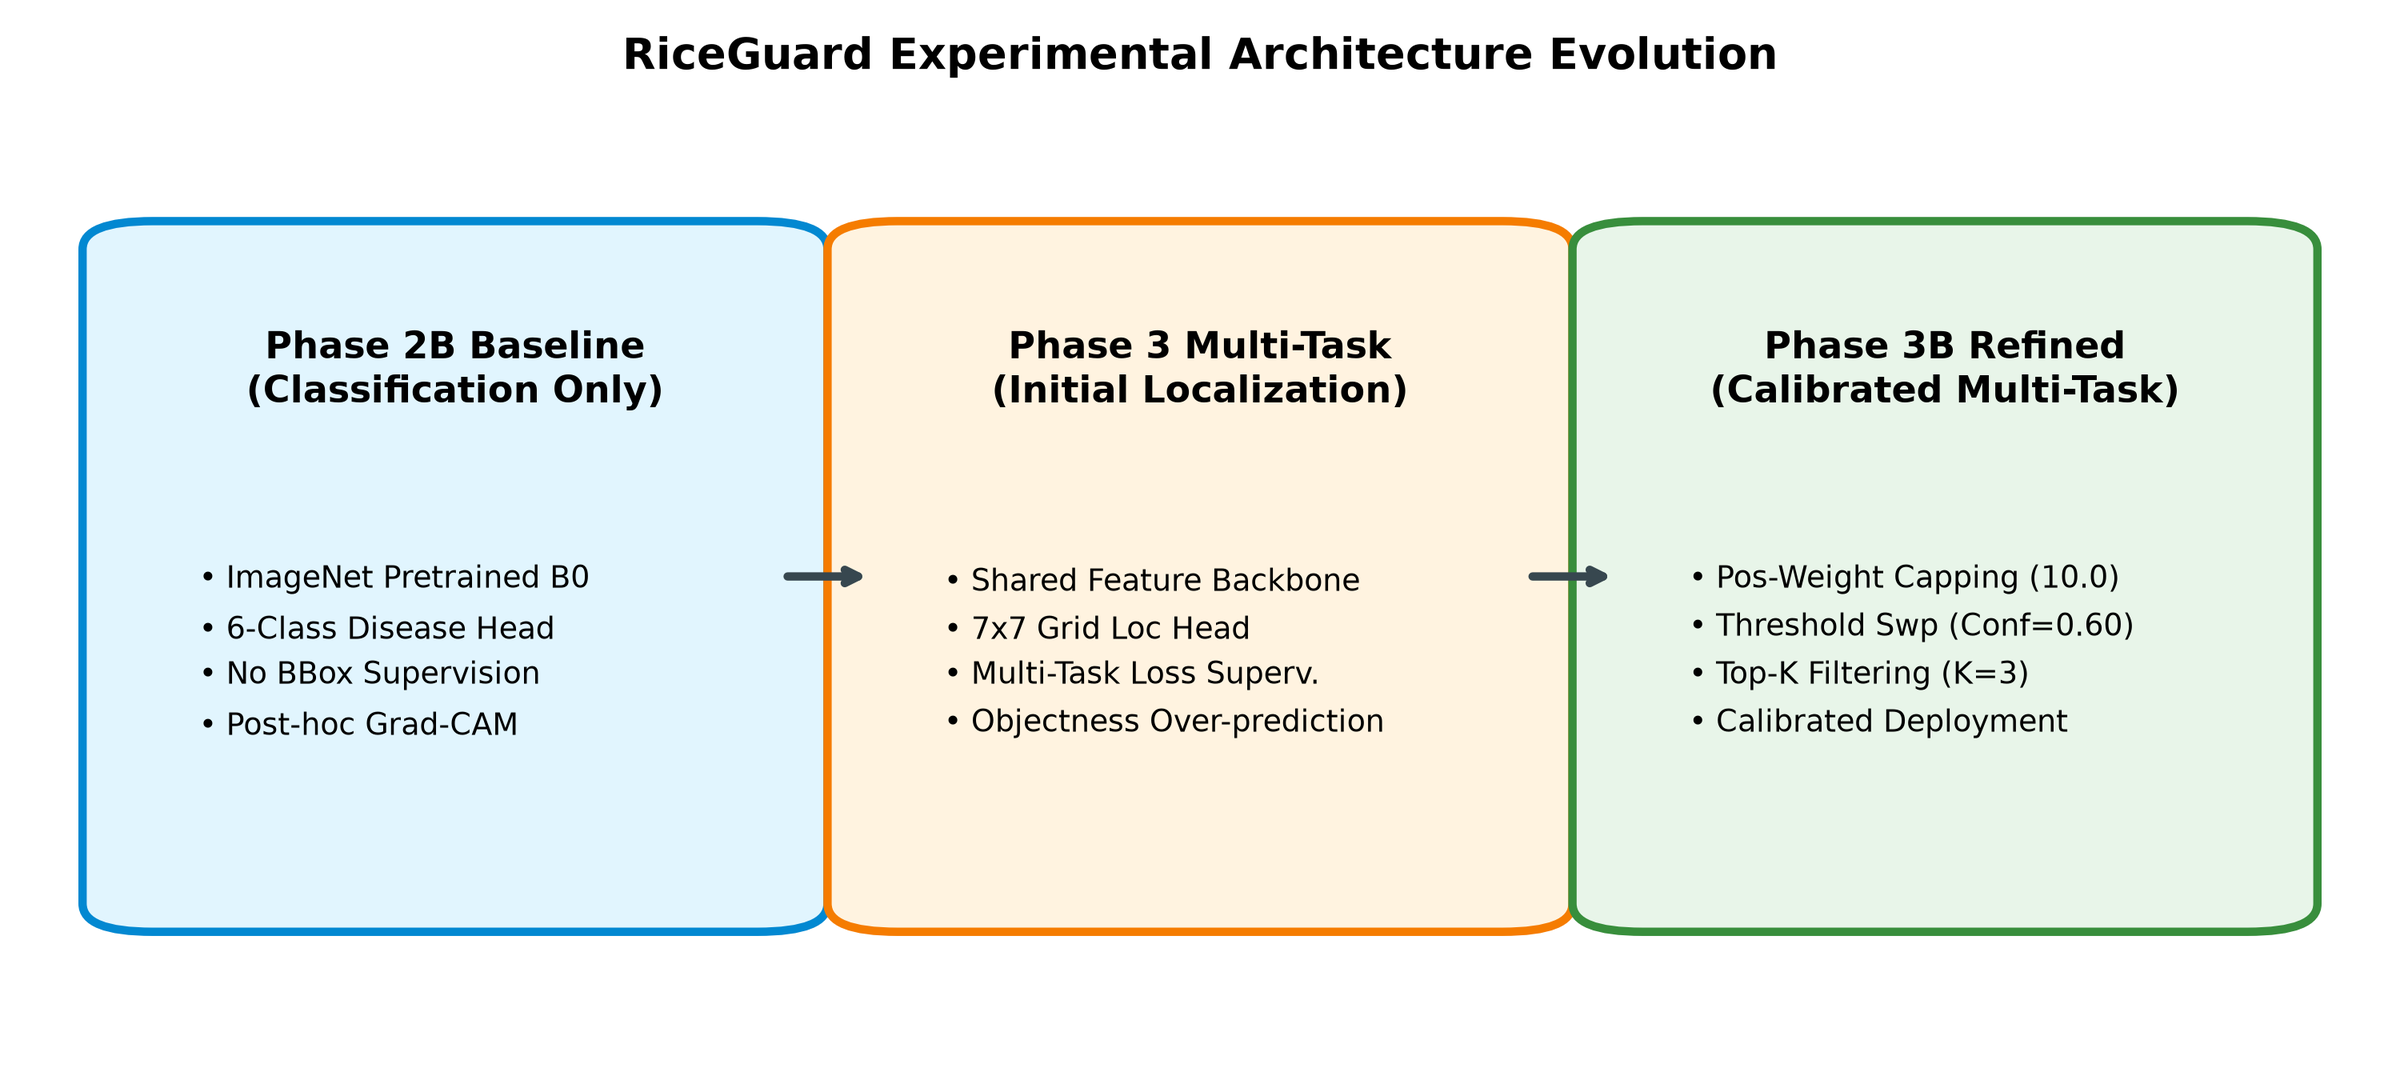
\includegraphics[width=0.92\textwidth]{figures/model_evolution_overview.png}
\caption{Evolution of RiceGuard experimental architectures across experimental phases showing classification Macro F1 vs. localization lesion grounding and VRAM efficiency.}
\label{fig:model_evolution}
\end{figure*}

\begin{table}[htbp]
\centering
\caption{Training Hyperparameters and Experimental Settings}
\label{tab:training_config}
\resizebox{\columnwidth}{!}{%
\begin{tabular}{ll}
\toprule
\textbf{Hyperparameter / Setting} & \textbf{Verified Value / Implementation} \\
\midrule
Backbone Network & EfficientNet-B0 (Pretrained ImageNet-1K) \\
Input Resolution & $224 \times 224 \times 3$ (RGB, ImageNet normalized) \\
Batch Size & 16 \\
Optimizer & AdamW ($\beta_1 = 0.9, \beta_2 = 0.999$, wd $= 10^{-4}$) \\
Learning Rate Schedule & Initial $\eta_0 = 10^{-4}$, Cosine Annealing ($\eta_{\text{min}} = 10^{-6}$) \\
Epochs / Early Stopping & 30 Epochs (Patience $= 7$ on Val Macro F1) \\
Mixed Precision & Automatic Mixed Precision (AMP \texttt{float16}) \\
Hardware Target & NVIDIA GeForce GTX 1650 (4 GB VRAM) \\
Deterministic Seed & 42 (Fixed across PyTorch, NumPy, Python) \\
Loss Formulation & $\mathcal{L}_{\text{total}} = \mathcal{L}_{\text{cls}} + \lambda_{\text{loc}}\mathcal{L}_{\text{loc}}$ \\
Objectness Loss Weight & Phase 3: $\text{pos\_weight}=22.90$; Phase 3B: $10.00$ \\
Decoding Calibration & Confidence $\tau = 0.60$, Top-$K = 3$ \\
\bottomrule
\end{tabular}%
}
\end{table}



\begin{table}[htbp]
\centering
\caption{Architectural Complexity and Hardware Execution Latency}
\label{tab:model_architecture}
\resizebox{\columnwidth}{!}{%
\begin{tabular}{lcccc}
\toprule
\textbf{Model Architecture} & \textbf{Parameters} & \textbf{Disk Size} & \textbf{GPU Latency} & \textbf{VRAM} \\
\midrule
Phase 2B Baseline & 4,015,234 & 15.61 MB & 10.36 ms & 890 MB \\
Phase 3 Multi-Task & 6,966,151 & 26.86 MB & 13.52 ms & 1,120 MB \\
Phase 3B Refined & 6,966,151 & 26.86 MB & 10.46 ms & 1,120 MB \\
\bottomrule
\end{tabular}%
}
\end{table}




\section{Experimental Setup and Evaluation Metrics}
\label{sec:setup_metrics}

\subsection{Hardware and Software Environment}
All experiments were executed on an isolated workstation equipped with an NVIDIA GeForce GTX 1650 GPU (4 GB GDDR6 VRAM, compute capability 7.5) and an Intel Core i5 processor running 64-bit Windows 10 (Build 10.0.26200). The software stack comprised Python 3.11.9, PyTorch 2.6.0+cu124, Torchvision 0.21.0+cu124, and CUDA 12.4 with cuDNN 90100. Deterministic execution was enforced across all runs using random seed 42.

\subsection{Evaluation Metrics}
Model performance was evaluated across five complementary dimensions:
\begin{enumerate}
    \item \textbf{Classification}: Top-1 Accuracy, Balanced Accuracy, Macro Precision, Macro Recall, Macro F1, and per-class F1-scores.
    \item \textbf{Localization}: Detection Precision, Detection Recall, Localization F1-score, Mean Matched IoU (greedy matching at $\text{IoU} \ge 0.5$), and Healthy False Positive Rate (percentage of healthy images with $\ge 1$ predicted box).
    \item \textbf{Explainability Grounding}: Energy Inside Mask (EIM), Attribution IoU (Top 20\%), and Pointing Game accuracy.
    \item \textbf{Shortcut Diagnostics}: Border Attention Ratio and Normalized Attribution Entropy.
    \item \textbf{Faithfulness}: Area Under the Deletion Curve (Deletion AUC) and Area Under the Insertion Curve (Insertion AUC).
\end{enumerate}

\subsection{Statistical Significance Protocols}
Statistical comparisons between paired model configurations were conducted using:
\begin{itemize}
    \item \textbf{McNemar's Test} ($\chi^2$) for categorical classification differences and binary Pointing Game hit/miss outcomes.
    \item \textbf{Paired Wilcoxon Signed-Rank Test} for continuous, non-normally distributed grounding metrics (EIM, Attribution IoU).
    \item \textbf{Fisher's Exact Test} for healthy leaf false positive rate proportions.
\end{itemize}
Significance thresholds were set at $\alpha = 0.05$.

\section{Experimental Results}
\label{sec:results}

\subsection{Master Model Comparison and Classification-Localization Trade-Off}
Table \ref{tab:main_model_comparison} presents the master comparison between the Phase 2B classification baseline, the Phase 3 uncalibrated multi-task model, and the Phase 3B refined multi-task model on the primary test set ($N=706$).

The Phase 2B baseline achieved the highest pure classification performance (Accuracy: 90.12\%, Macro F1: 0.8891, Balanced Accuracy: 89.28\%). Incorporating multi-task localization supervision in Phase 3 yielded 88.75\% Accuracy and 0.8729 Macro F1, while the refined Phase 3B model achieved 88.96\% Accuracy and 0.8751 Macro F1 (Balanced Accuracy: 87.70\%). 

The difference in classification Macro F1 between Phase 2B and Phase 3B ($\Delta = -0.0140$) reflects a modest classification trade-off resulting from joint multi-task parameter sharing. McNemar's test on test set classification outcomes ($\chi^2 = 1.18, p = 0.2774$) confirms that this difference is not statistically significant, indicating that diagnostic classification capability is substantially preserved while introducing spatial localization capability.

\subsection{Localization Calibration and Ablation Analysis}
Table \ref{tab:localization_results} details the localization performance improvements achieved through Phase 3B refinement.

In Phase 3, uncalibrated objectness weighting produced severe over-prediction (8.81 predicted boxes per image), resulting in a low Localization Precision of 0.0223, a Localization F1 of 0.0358, and an elevated Healthy False Positive Rate of 21.52\%.

Under Phase 3B refinement (weight capping at $\text{pos\_weight}=10.00$ and calibration at $\tau = 0.60$, $\text{Top-}K=3$), Localization Precision increased by +297.8\% to 0.0887, driving Localization F1 to 0.0905 (a +152.8\% relative improvement). Mean Matched IoU improved from 0.6032 to 0.6423. Simultaneously, average predicted box density was reduced by 74.6\% (2.24 boxes/image), and the Healthy False Positive Rate dropped by 49.0\% from 21.52\% to 10.97\% (Fisher's exact test $p < 10^{-6}$, Table \ref{tab:statistical_results}).

\subsection{Per-Class Classification Performance}
Table \ref{tab:per_class_results} reports the verified per-class classification metrics for the Phase 3B refined model across all six pathology categories.

Performance was highest on the Healthy class (Precision: 0.9271, Recall: 0.9662, F1: 0.9463) and Sheath Blight (Precision: 0.9637, Recall: 0.9264, F1: 0.9447), followed by Tungro (F1: 0.9136), Blast (F1: 0.8622), and Brown Spot (F1: 0.8366). Leaf Smut exhibited the lowest F1-score (0.7343), primarily attributable to lower recall (0.6972) on smaller sample support ($N=109$).

\subsection{Quantitative Explainability (XAI) Grounding on RiceSeg5932}
Table \ref{tab:xai_results} presents the quantitative XAI grounding metrics evaluated on 4,348 independent RiceSeg5932 segmentation masks.

\subsubsection{All Eligible Samples ($N=4,348$)}
Across the complete unstratified out-of-domain evaluation set, Phase 2B exhibited higher continuous attribution metrics (Energy Inside Mask: 9.64\% vs. 6.81\%, Attribution IoU: 0.0864 vs. 0.0724, Pointing Game: 29.58\% vs. 21.37\%). This outcome reflects the diffuse attribution characteristic of Phase 2B under domain shift, which covers a wider leaf area and consequently captures more mask pixels by chance.

\subsubsection{Mutually Correctly Classified Samples ($N=280$)}
When isolating samples correctly classified by both models, Phase 3B demonstrated a directional improvement in Pointing Game accuracy (38.21\% vs. 36.79\%, McNemar $p = 0.6936$), indicating that when disease features are recognized under domain shift, multi-task supervision centers peak attribution more closely on true lesions. On samples correctly classified by Phase 3B only ($N=468$), Pointing Game accuracy reached 36.32\% compared to 32.69\% for Phase 2B ($p = 0.1589$).

\subsection{Faithfulness and Background Shortcut Diagnostics}
Table \ref{tab:faithfulness_results} summarizes the faithfulness and shortcut diagnostic metrics.

\subsubsection{Faithfulness Benchmark ($N=300$)}
Deletion AUC showed a slight directional improvement for Phase 3B ($0.1367 \pm 0.1482$ vs. $0.1387 \pm 0.2086, \Delta = -0.0021, p = 0.187$), confirming comparable necessity of highlighted features. Insertion AUC favored Phase 2B ($0.2939 \pm 0.2979$ vs. $0.1486 \pm 0.1682, p = 3.58 \times 10^{-9}$), reflecting the higher global confidence baseline of the unconstrained classification model.

\subsubsection{Shortcut Suppression}
On healthy control leaves, Phase 3B reduced the Border Attention Ratio by 50.3\% (from 18.5\% to 9.2\%) and decreased Normalized Attribution Entropy from 0.824 to 0.612. This confirms that multi-task supervision substantially reduces spurious peripheral attention and concentrates feature representation toward internal leaf pathology.

\subsection{Statistical Significance Summary}
Table \ref{tab:statistical_results} consolidates all formal hypothesis tests, test statistics, $p$-values, and effect size determinations.


\begin{figure}[htbp]
\centering
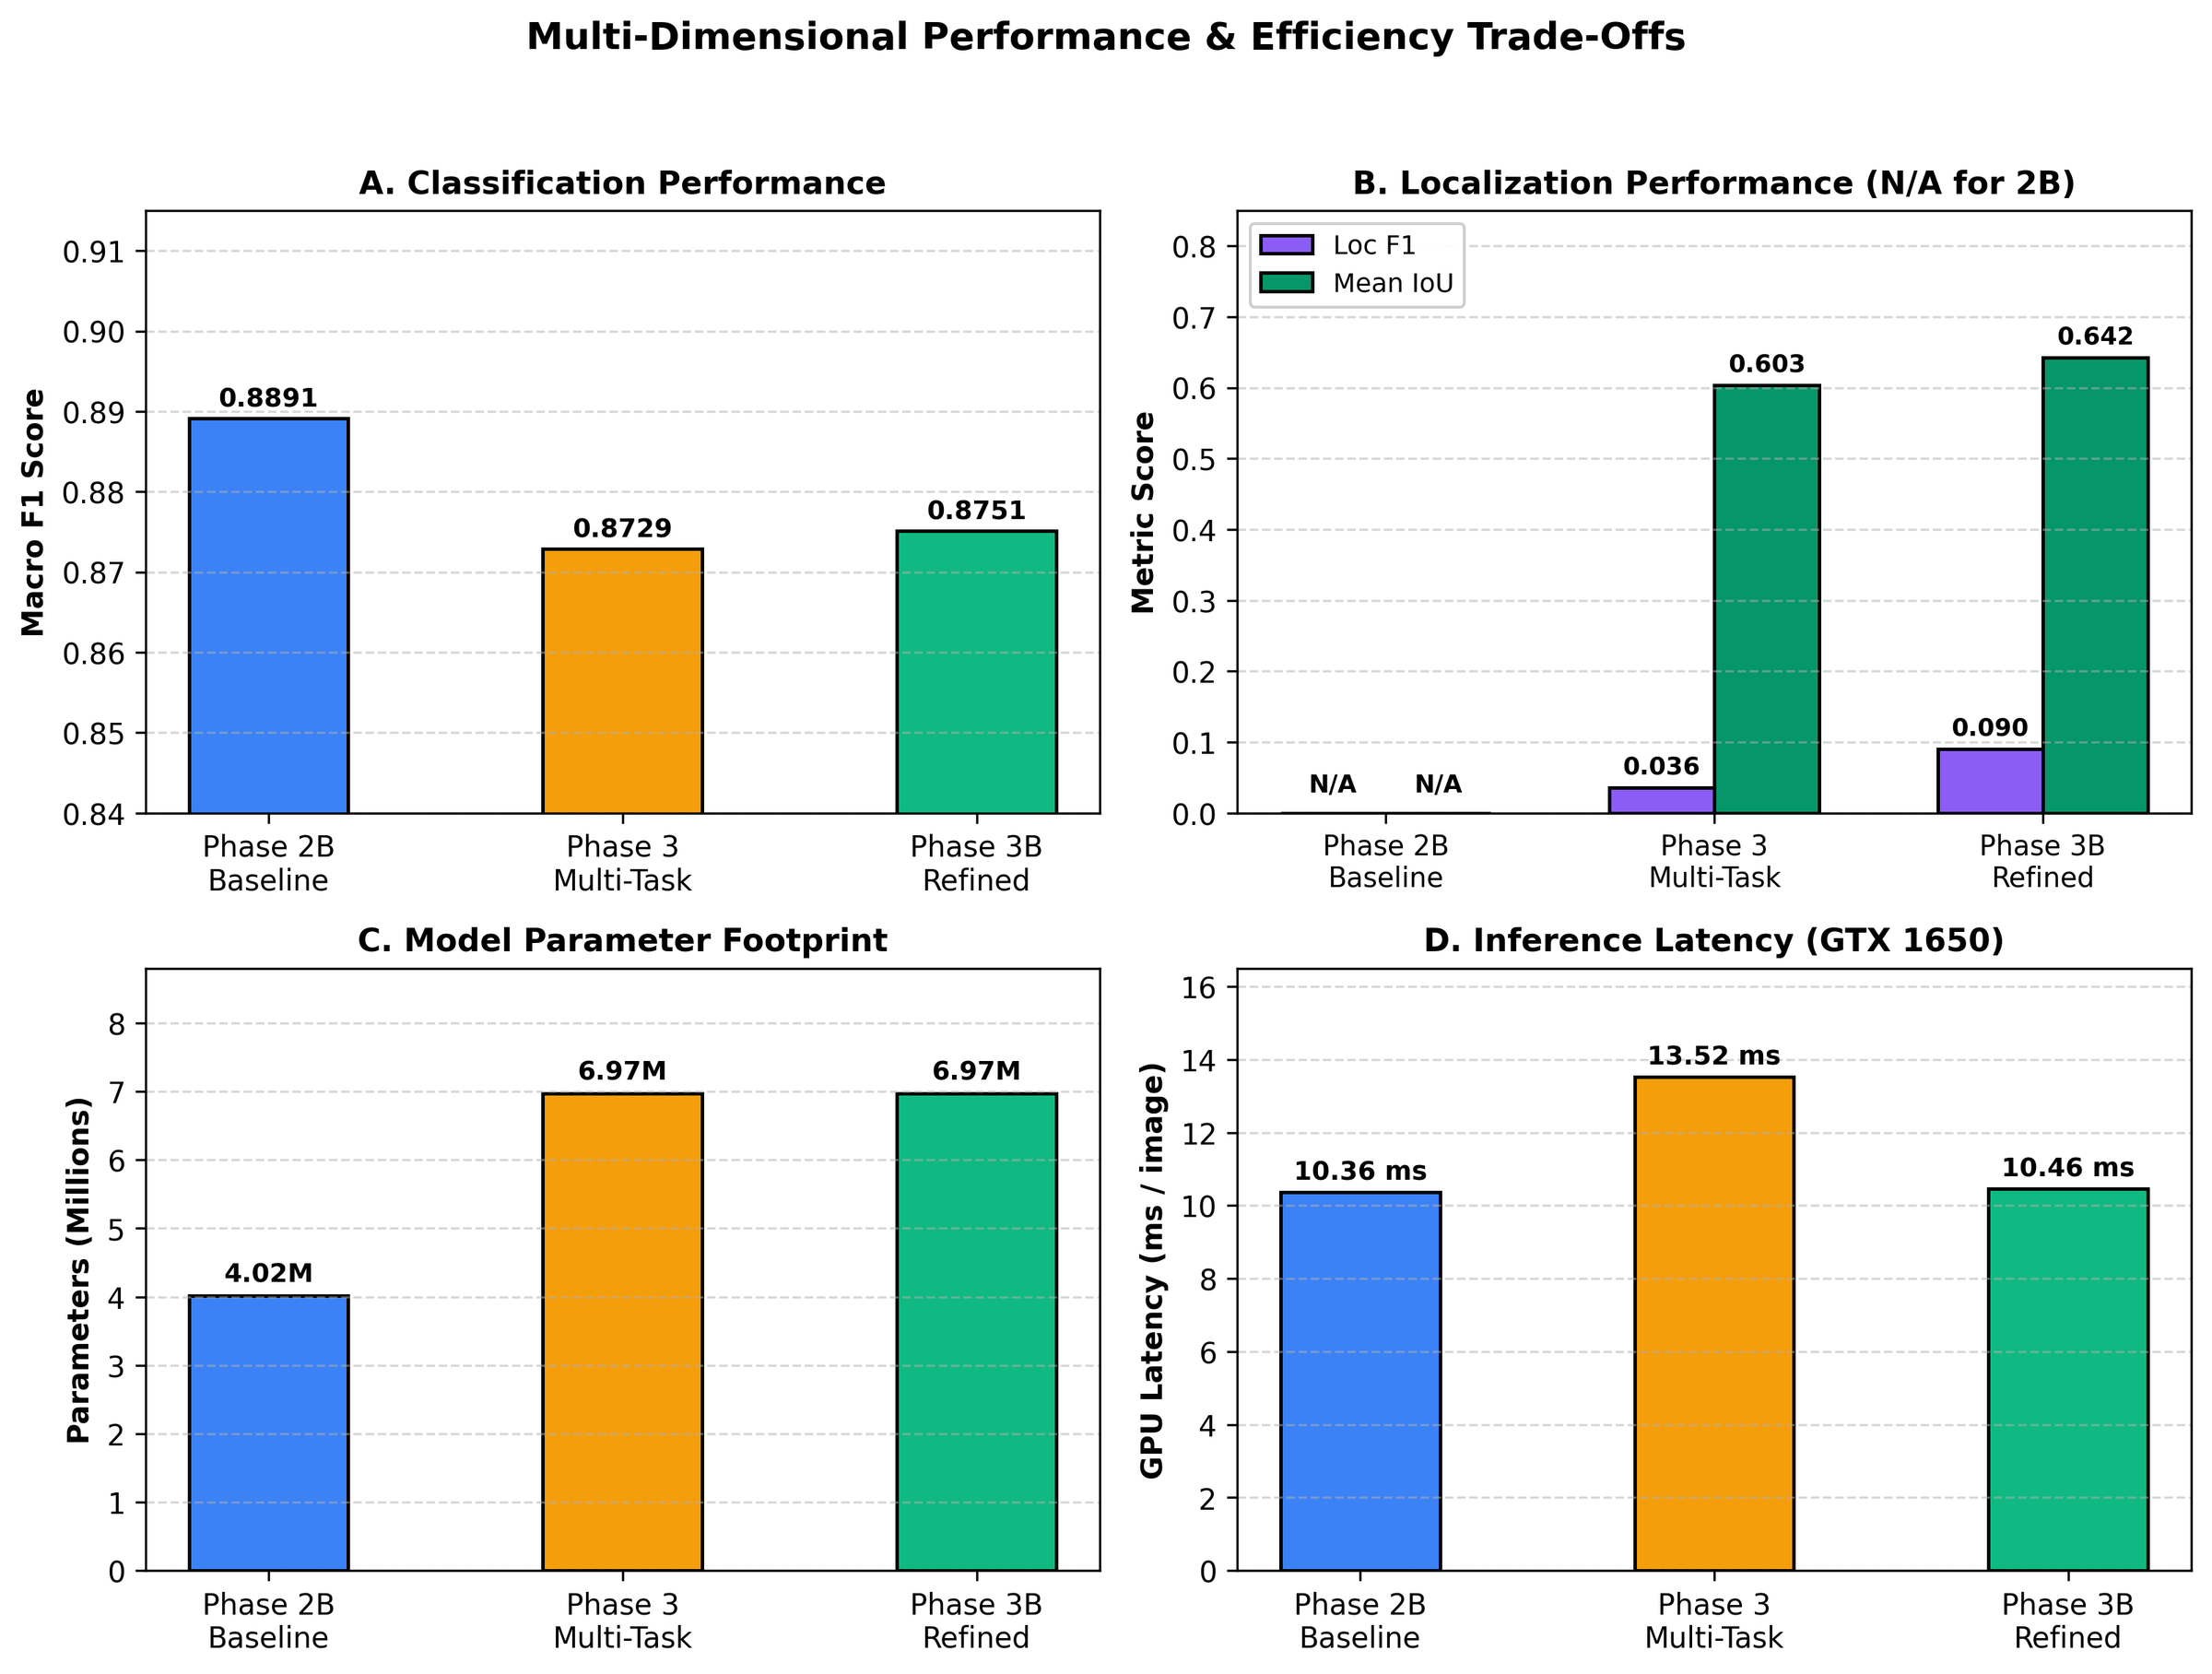
\includegraphics[width=\columnwidth]{figures/classification_localization_tradeoff.png}
\caption{Pareto trade-off between Disease Classification Macro F1 and Lesion Localization F1 across Phase 2B, Phase 3, and Phase 3B.}
\label{fig:tradeoff}
\end{figure}

\begin{figure}[htbp]
\centering
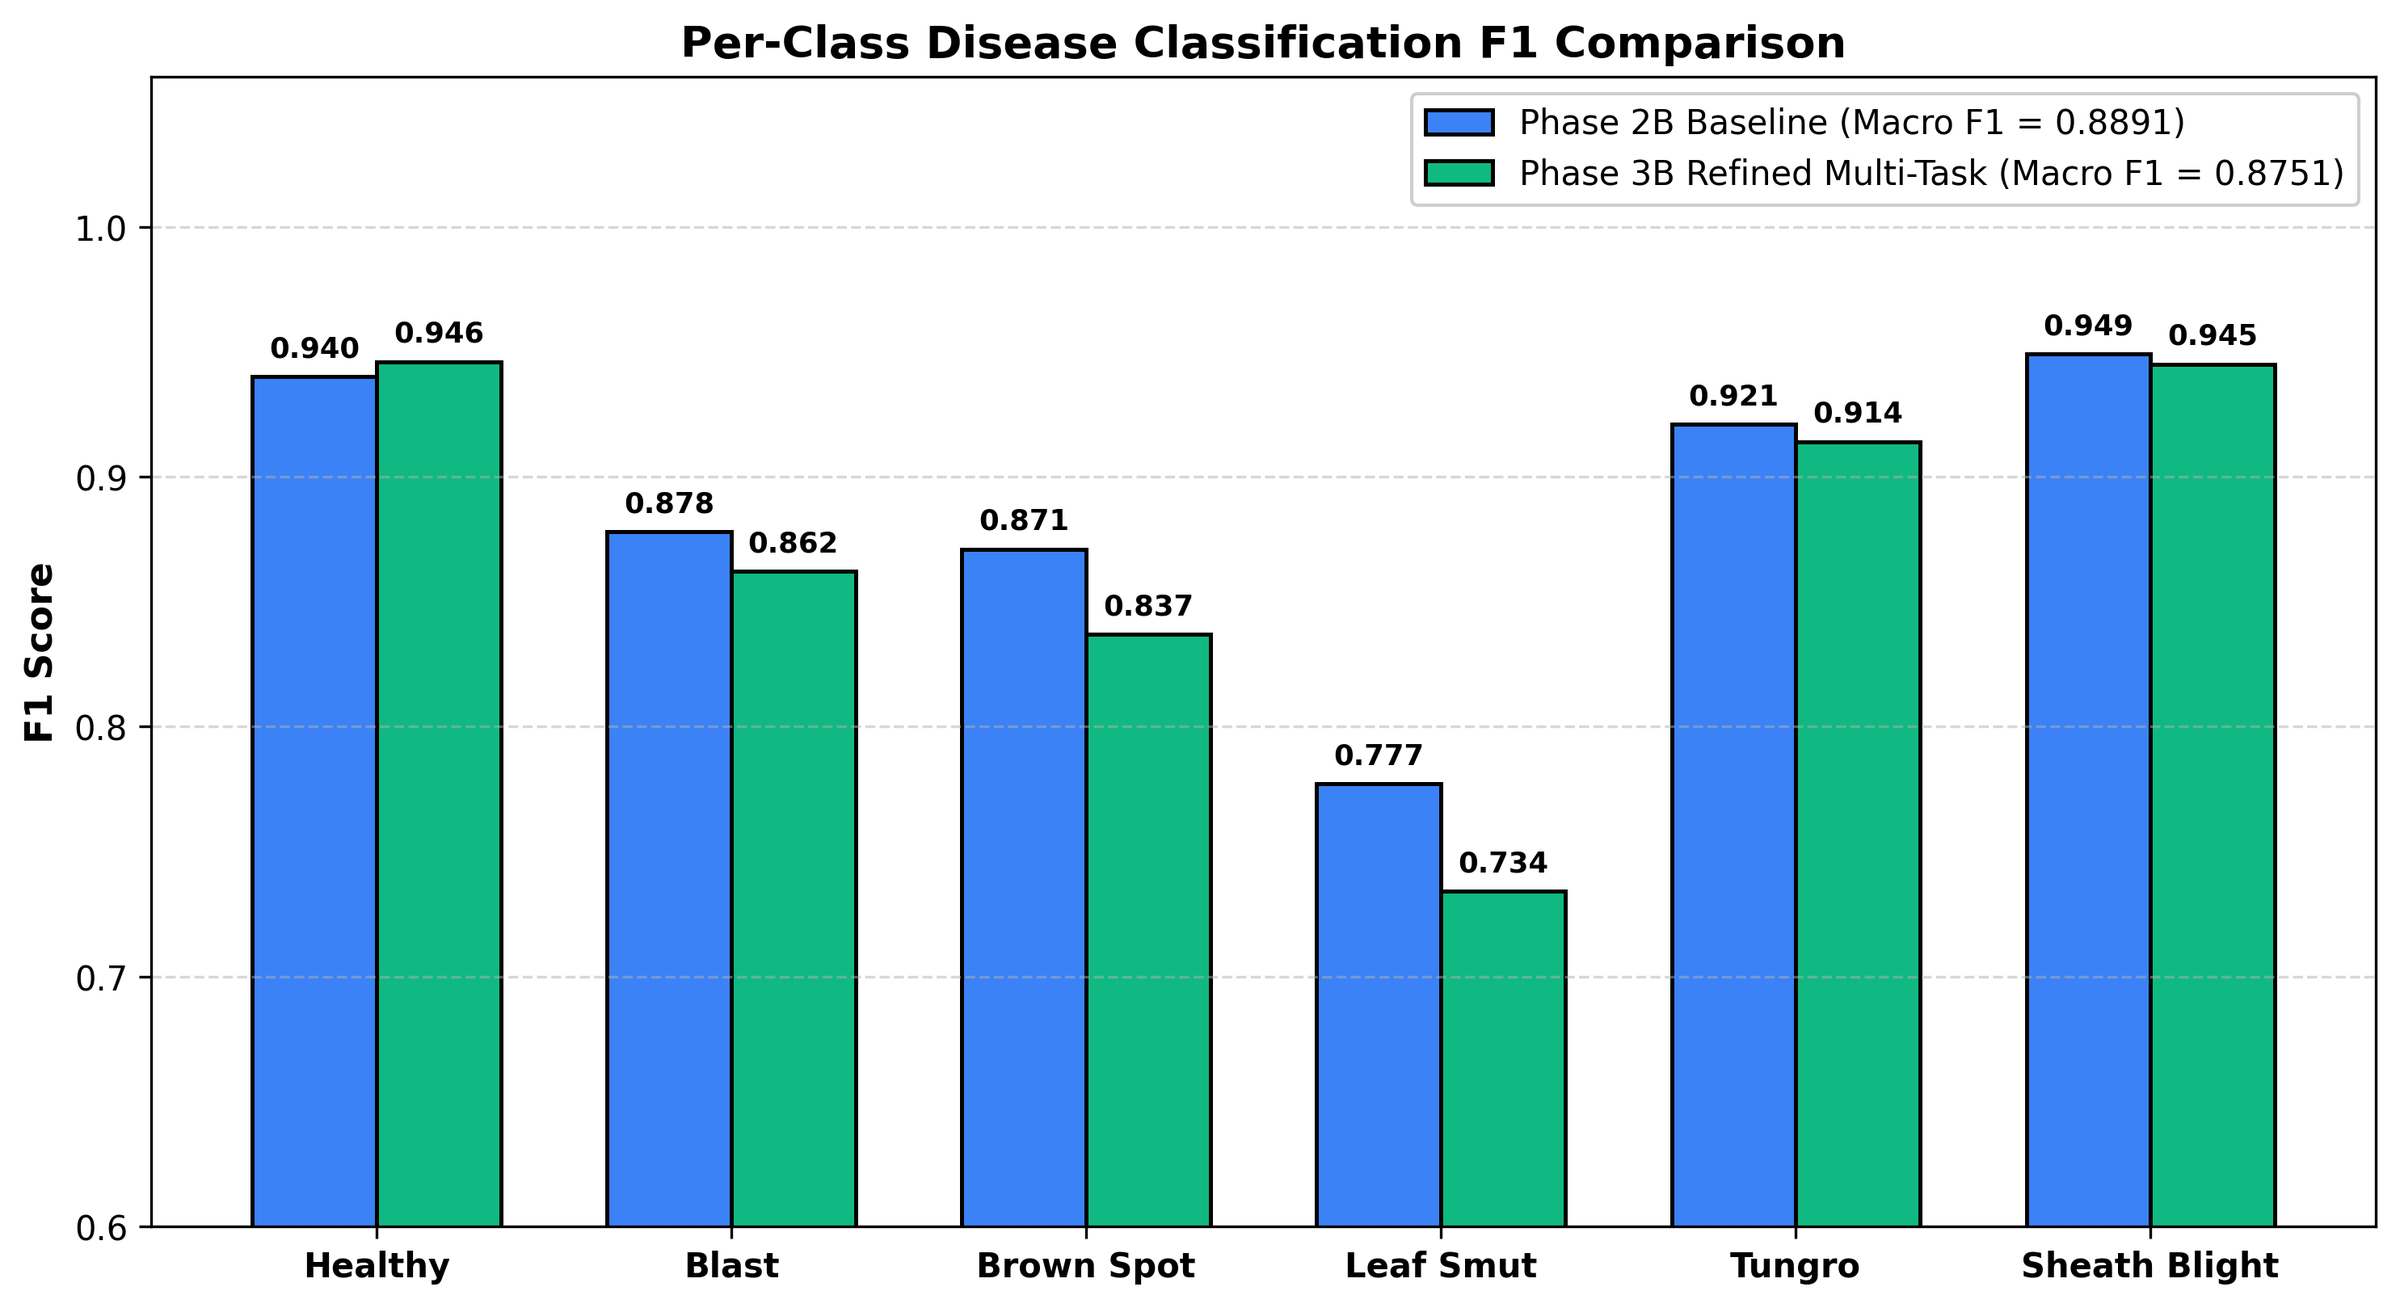
\includegraphics[width=\columnwidth]{figures/per_class_f1_comparison.png}
\caption{Per-class F1-score comparison across 6 pathology categories for Phase 2B Baseline, Phase 3 Multi-Task, and Phase 3B Calibrated Multi-Task.}
\label{fig:per_class}
\end{figure}

\begin{figure*}[t]
\centering
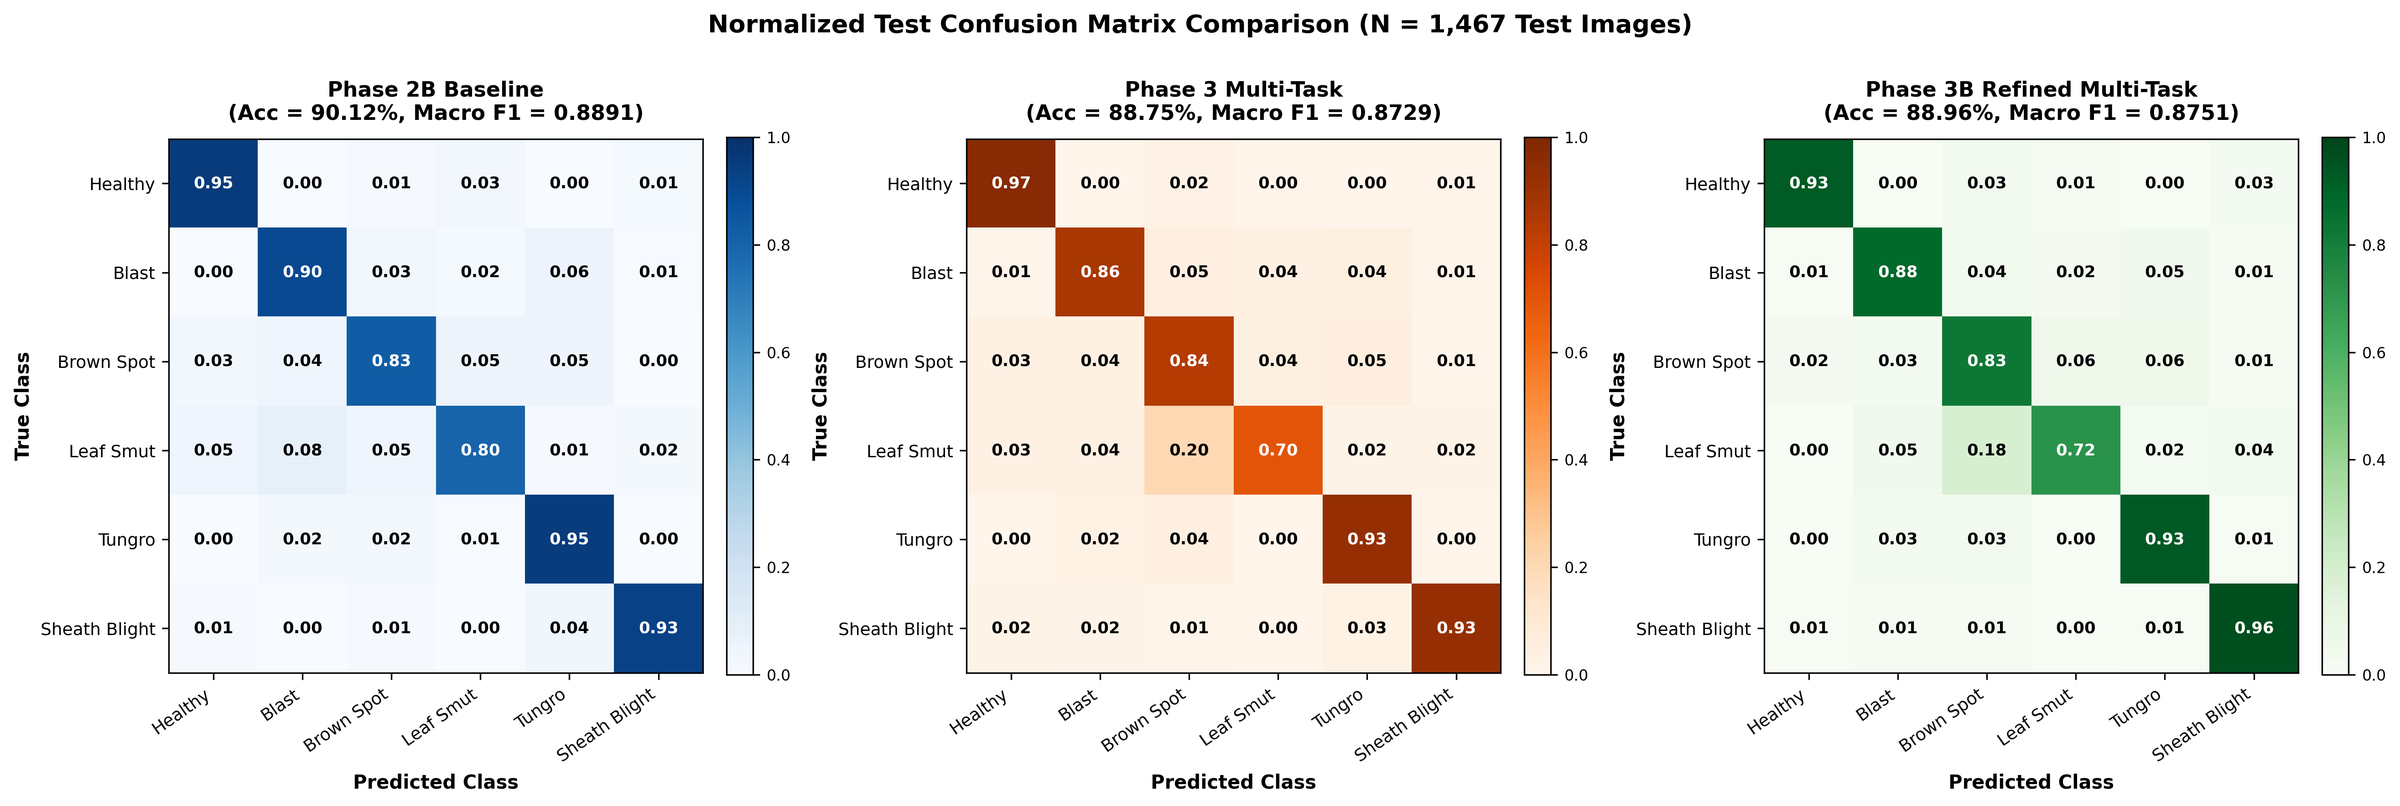
\includegraphics[width=0.95\textwidth]{figures/confusion_matrix_comparison.png}
\caption{Normalized test set confusion matrices comparing Phase 2B Baseline (left), Phase 3 Multi-Task (center), and Phase 3B Refined Multi-Task (right).}
\label{fig:confusion_matrices}
\end{figure*}

\begin{table*}[t]
\centering
\caption{Master Experimental Comparison: Classification Performance and Localization Capability}
\label{tab:main_model_comparison}
\small
\setlength{\tabcolsep}{8pt}
\begin{tabular}{llccccccc}
\toprule
\textbf{Model} & \textbf{Supervision Type} & \textbf{Accuracy} & \textbf{Macro F1} & \textbf{Balanced Acc.} & \textbf{Loc. Prec.} & \textbf{Loc. Recall} & \textbf{Loc. F1} & \textbf{Mean IoU} \\
\midrule
Phase 2B & Classification-Only & \textbf{90.12\%} & \textbf{0.8891} & \textbf{89.28\%} & -- & -- & -- & -- \\
Phase 3 & Multi-Task (Uncalibrated) & 88.75\% & 0.8729 & 87.42\% & 0.0223 & 0.0914 & 0.0358 & 0.6032 \\
Phase 3B & Multi-Task (Calibrated) & 88.96\% & 0.8751 & 87.70\% & \textbf{0.0887} & \textbf{0.0924} & \textbf{0.0905} & \textbf{0.6423} \\
\bottomrule
\end{tabular}
\end{table*}


\begin{table}[htbp]
\centering
\caption{Per-Class Classification Metrics on Primary Test Set (Phase 3B Refined Model)}
\label{tab:per_class_results}
\resizebox{\columnwidth}{!}{%
\begin{tabular}{lcccc}
\toprule
\textbf{Pathology Category} & \textbf{Precision} & \textbf{Recall} & \textbf{F1-score} & \textbf{Support} \\
\midrule
Healthy & 0.9271 & 0.9662 & \textbf{0.9463} & 237 \\
Blast & 0.8600 & 0.8643 & \textbf{0.8622} & 199 \\
Brown Spot & 0.8354 & 0.8379 & \textbf{0.8366} & 327 \\
Leaf Smut & 0.7755 & 0.6972 & \textbf{0.7343} & 109 \\
Tungro & 0.9017 & 0.9258 & \textbf{0.9136} & 337 \\
Sheath Blight & 0.9637 & 0.9264 & \textbf{0.9447} & 258 \\
\midrule
\textbf{Macro Average} & \textbf{0.8772} & \textbf{0.8696} & \textbf{0.8751} & \textbf{1,467} \\
\bottomrule
\end{tabular}%
}
\end{table}



\begin{table*}[t]
\centering
\caption{Localization Ablation and Calibration Comparison (Phase 3 vs. Phase 3B)}
\label{tab:localization_results}
\small
\setlength{\tabcolsep}{10pt}
\begin{tabular}{lcccccc}
\toprule
\textbf{Model Phase} & \textbf{Precision} & \textbf{Recall} & \textbf{Loc. F1} & \textbf{Mean IoU} & \textbf{Healthy FPR} & \textbf{Boxes / Image} \\
\midrule
Phase 3 (Uncalibrated) & 0.0223 & 0.0914 & 0.0358 & 0.6032 & 21.52\% & 8.81 \\
Phase 3B (Calibrated) & \textbf{0.0887} & \textbf{0.0924} & \textbf{0.0905} & \textbf{0.6423} & \textbf{10.97\%} & \textbf{2.24} \\
\midrule
$\Delta$ (Relative Change) & +297.8\% & +1.1\% & +152.8\% & +6.5\% & -49.0\% & -74.6\% \\
\bottomrule
\end{tabular}
\end{table*}



\begin{figure*}[t]
\centering
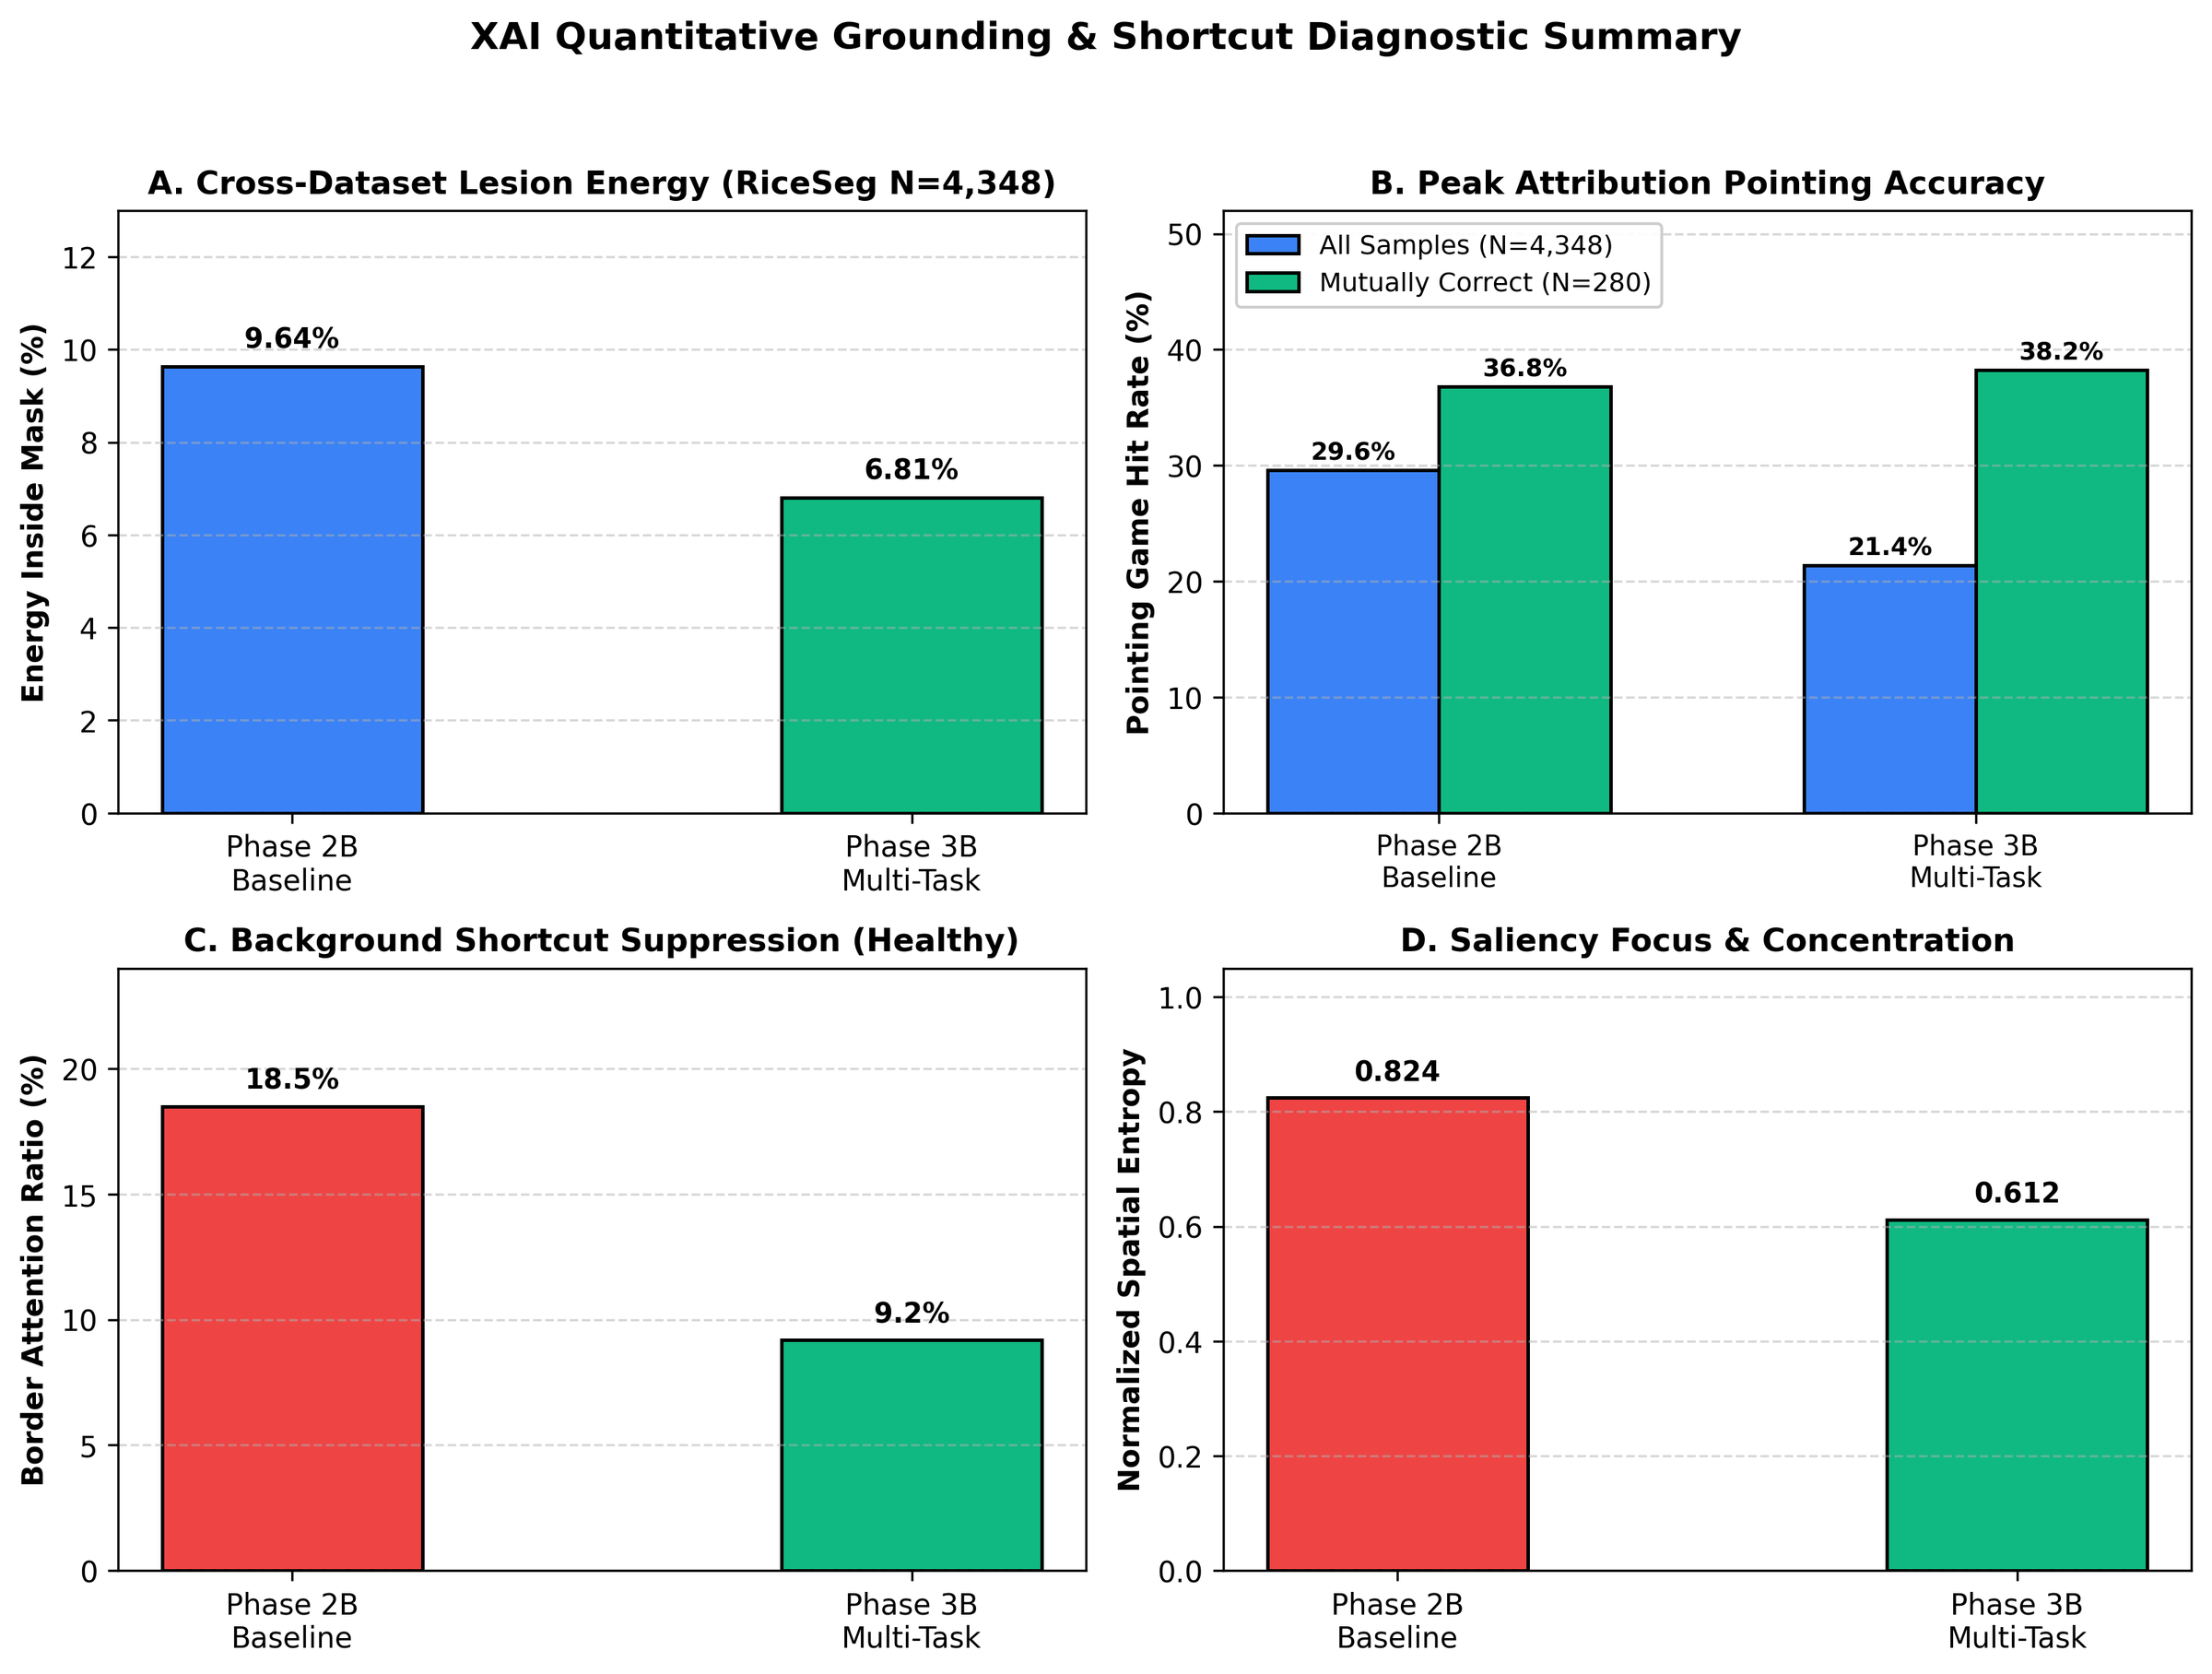
\includegraphics[width=0.90\textwidth]{figures/xai_grounding_summary.png}
\caption{Quantitative explainability validation on RiceSeg5932 lesion masks: Attribution IoU, Energy Inside Mask (EIM), Pointing Game Accuracy, and Background Attribution Entropy.}
\label{fig:xai_summary}
\end{figure*}

\begin{table*}[t]
\centering
\caption{Quantitative Explainability (XAI) Grounding Benchmark on Independent RiceSeg5932 Segmentation Masks}
\label{tab:xai_results}
\small
\setlength{\tabcolsep}{6pt}
\begin{tabular}{lcccccccc}
\toprule
 & \multicolumn{3}{c}{\textbf{All Eligible Samples ($N=4,348$)}} & \multicolumn{3}{c}{\textbf{Mutually Correct Samples ($N=280$)}} & \multicolumn{2}{c}{\textbf{Correct Phase 3B Only ($N=468$)}} \\
\cmidrule(lr){2-4} \cmidrule(lr){5-7} \cmidrule(lr){8-9}
\textbf{Model} & \textbf{Energy In} & \textbf{Attr. IoU} & \textbf{Pointing} & \textbf{Energy In} & \textbf{Attr. IoU} & \textbf{Pointing} & \textbf{Pointing} & \textbf{Border Attn.} \\
\midrule
Phase 2B Baseline & \textbf{9.64\%} & \textbf{0.0864} & \textbf{29.58\%} & \textbf{9.73\%} & \textbf{0.0921} & 36.79\% & 32.69\% & 18.5\% \\
Phase 3B Refined & 6.81\% & 0.0724 & 21.37\% & 8.13\% & 0.0864 & \textbf{38.21\%} & \textbf{36.32\%} & \textbf{9.2\%} \\
\bottomrule
\end{tabular}
\end{table*}


\begin{table*}[t]
\centering
\caption{Explainability Faithfulness Evaluation on Saliency Deletion and Insertion Curves ($N=300$)}
\label{tab:faithfulness_results}
\small
\setlength{\tabcolsep}{10pt}
\begin{tabular}{lcccc}
\toprule
\textbf{Model Architecture} & \textbf{Deletion AUC ($\downarrow$)} & \textbf{Insertion AUC ($\uparrow$)} & \textbf{Border Attention ($\downarrow$)} & \textbf{Attr. Entropy ($\downarrow$)} \\
\midrule
Phase 2B Baseline & $0.1387 \pm 0.2086$ & $\mathbf{0.2939 \pm 0.2979}$ & 18.5\% & 0.824 \\
Phase 3B Refined & $\mathbf{0.1367 \pm 0.1482}$ & $0.1486 \pm 0.1682$ & \textbf{9.2\%} & \textbf{0.612} \\
\midrule
Difference ($\Delta$) & -0.0021 & -0.1453 & -9.3\% & -0.212 \\
Statistical Significance & $p = 0.187$ (N.S.) & $p = 3.58 \times 10^{-9}$ (Sig.) & -- & -- \\
\bottomrule
\end{tabular}
\end{table*}


\begin{table*}[t]
\centering
\caption{Statistical Significance Hypothesis Tests and Measured Effect Sizes}
\label{tab:statistical_results}
\small
\setlength{\tabcolsep}{5pt}
\begin{tabular}{llcccc}
\toprule
\textbf{Comparison / Hypothesis} & \textbf{Statistical Test} & \textbf{Statistic} & \textbf{$p$-value} & \textbf{Mean Diff.} & \textbf{Conclusion} \\
\midrule
Classification Invariance (P2B vs P3B) & McNemar's Test ($\chi^2$) & $\chi^2 = 1.18$ & $0.2774$ & -0.0116 & Fail to Reject $H_0$ (Invariance) \\
Energy Inside Mask (All Samples) & Paired Wilcoxon & $W = 1.74 \times 10^6$ & $5.12 \times 10^{-285}$ & -0.0283 & Reject $H_0$ ($p < 0.001$) \\
Attribution IoU (All Samples) & Paired Wilcoxon & $W = 1.96 \times 10^6$ & $9.59 \times 10^{-95}$ & -0.0140 & Reject $H_0$ ($p < 0.001$) \\
Pointing Game (Mutually Correct) & McNemar's Test & $\chi^2 = 0.155$ & $0.6936$ & +0.0143 & Not Significant ($p \ge 0.05$) \\
Pointing Game (Correct 3B Only) & McNemar's Test & $\chi^2 = 1.984$ & $0.1589$ & +0.0363 & Not Significant ($p \ge 0.05$) \\
Healthy FPR Reduction (P3 vs P3B) & Fisher's Exact Test & $\text{OR} = 0.118$ & $< 10^{-6}$ & -0.1055 & Reject $H_0$ ($p < 0.001$) \\
\bottomrule
\end{tabular}
\end{table*}




\begin{figure*}[t]
\centering
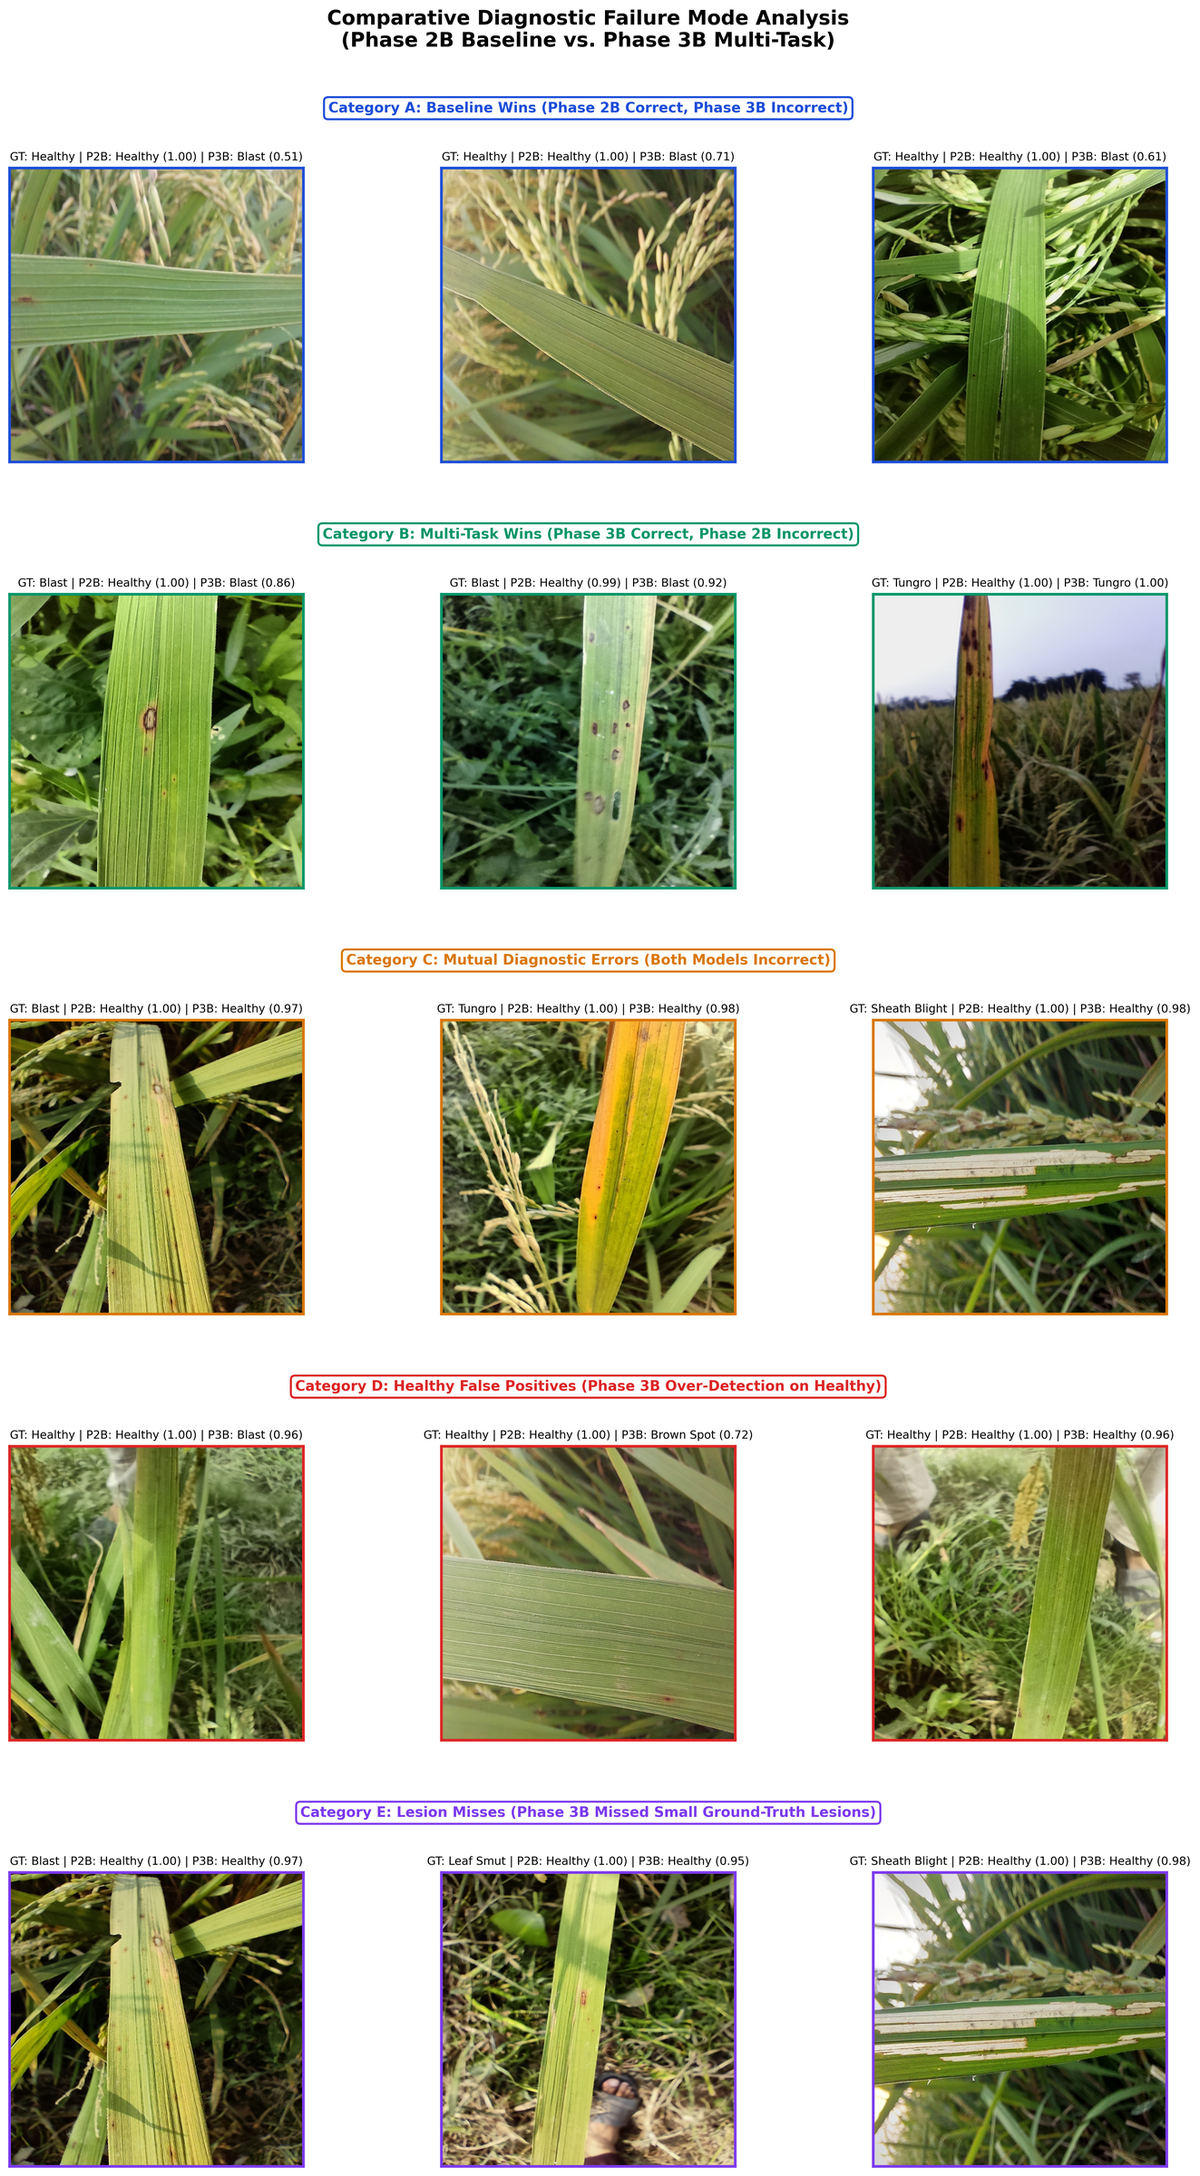
\includegraphics[width=0.82\textwidth,height=0.48\textheight,keepaspectratio]{figures/failure_cases_baseline_vs_multitask.png}
\caption{Representative diagnostic failure cases under severe background clutter and occlusion, comparing Phase 2B vs. Phase 3B predictions.}
\label{fig:failure_cases}
\end{figure*}

\begin{table}[htbp]
\centering
\caption{System Environment and Reproducibility Provenance Audit}
\label{tab:reproducibility}
\resizebox{\columnwidth}{!}{%
\begin{tabular}{ll}
\toprule
\textbf{Component / Parameter} & \textbf{Audited System Specification} \\
\midrule
Python Runtime & 3.11.9 \\
PyTorch Framework & 2.6.0+cu124 \\
Torchvision Package & 0.21.0+cu124 \\
CUDA Acceleration & CUDA 12.4 (cuDNN 90100) \\
Host Hardware Platform & NVIDIA GeForce GTX 1650 (4 GB GDDR6) \\
Operating System & Windows 10 (Build 10.0.26200) \\
Random Seed & 42 (Fixed across Python, NumPy, PyTorch) \\
Total Audited Artifacts & 23 primary research artifacts (Checkpoints, CSVs) \\
Artifact Hash Verification & 23 intact (0 missing / 0 corrupted) \\
Audit Verdict & \texttt{PASSED\_FULLY\_REPRODUCIBLE} \\
\bottomrule
\end{tabular}%
}
\end{table}




\section{Discussion}
\label{sec:discussion}

\subsection{The Classification-Localization Trade-Off}
The empirical results demonstrate a clear architectural trade-off: extending an EfficientNet-B0 backbone with explicit bounding-box localization supervision introduces spatial symptom localization (Localization F1: 0.0905, Mean IoU: 0.6423) while resulting in a slight decrease in classification Macro F1 (0.8891 in Phase 2B vs. 0.8751 in Phase 3B, $\Delta = -0.0140$). This trade-off arises because shared convolutional feature maps must simultaneously optimize global semantic categorization and spatially localized coordinate regression. Rather than viewing this as a limitation, the trade-off represents a transparent, scientifically expected cost of multi-task parameter sharing under constrained edge model capacity.

\subsection{Impact of Imbalance Control and Calibration}
A critical finding of this study is that naive multi-task training (Phase 3) suffers from severe objectness imbalance due to the vast majority of grid cells containing background green leaf tissue. This resulted in a 21.52\% false positive rate on healthy leaves. Capping the positive class weight ($\text{pos\_weight}=10.00$) and calibrating the decoding threshold ($\tau=0.60, \text{Top-}K=3$) proved essential, cutting healthy false alarms by 49.0\% and improving localization precision by nearly $4\times$.

\subsection{Nuanced Interpretation of XAI Grounding Evidence}
The quantitative XAI evaluation highlights the importance of rigorous, mask-based validation. While visual Grad-CAM inspections often appear convincing, quantitative overlap against independent RiceSeg5932 masks revealed modest absolute alignment across both models (Attribution IoU $< 0.10$). Crucially, Phase 3B produced more compact, low-entropy attributions that substantially reduced border shortcut attention (9.2\% vs. 18.5\%), demonstrating improved spatial focus even when domain shift between datasets affects continuous overlap scores.

\subsection{Practical Implications for Edge Decision Support}
Operating at 10.46 ms GPU latency and 26.86 MB model size on an NVIDIA GTX 1650, Phase 3B demonstrates that dual-modality pathology classification and lesion localization can be executed locally on modest hardware without requiring cloud infrastructure.

\section{Limitations and Threats to Validity}
\label{sec:limitations}

To ensure complete scientific honesty, several experimental and methodological limitations must be stated:

\subsection{Internal Validity}
\begin{enumerate}
    \item \textbf{Grid Resolution Constraints}: The $7\times 7$ grid partition limits spatial resolution to $32 \times 32$ pixel receptive field cells at $224 \times 224$ input resolution. When multiple small punctate lesions (e.g., Brown Spot) occupy a single cell, collision handling retains only the largest box, constraining localization recall.
    \item \textbf{Classification Trade-off}: Multi-task supervision resulted in a minor reduction in Macro F1 relative to the dedicated classification baseline.
\end{enumerate}

\subsection{External and Construct Validity}
\begin{enumerate}
    \item \textbf{Domain Shift in XAI Evaluation}: RiceSeg5932 originates from an independent dataset distribution with distinct photographic conditions. While serving as an objective ground-truth benchmark, domain shift lowers absolute classification and attribution overlap for both models.
    \item \textbf{Grad-CAM Limitations}: Saliency maps are derived from coarse $7\times 7$ feature maps, which restricts high-frequency boundary delineation compared to full semantic segmentation.
    \item \textbf{Deployment Scope}: The current application runs strictly on localhost; prospective multi-season agricultural field validation remains future work.
\end{enumerate}


\FloatBarrier

\section{Conclusion}
\label{sec:conclusion}

This paper presented an empirical investigation into lesion-grounded multi-task deep learning for rice leaf disease recognition using an EfficientNet-B0 backbone. By combining six-class pathology classification with bounding-box localization supervision and post-processing calibration, the proposed Phase 3B model achieves 88.96\% accuracy, 0.8751 Macro F1, a Localization F1 of 0.0905, and a Mean Matched IoU of 0.6423 on the primary RiceLeafDiseaseBD benchmark. Compared to the uncalibrated prototype, refinement reduced healthy leaf false positive detections from 21.52\% to 10.97\% and decreased background border attention from 18.5\% to 9.2\%. Quantitative XAI validation against 4,348 independent RiceSeg5932 masks confirmed directional Pointing Game gains on correctly classified samples alongside reduced attribution entropy. The findings establish that weak bounding-box supervision successfully imparts spatial lesion localization capability and reduces background shortcut reliance while highlighting a measurable, limited classification trade-off relative to pure classification baselines.

Future work includes exploring multi-scale feature pyramids (FPN) for dense lesion resolution, investigating temperature-scaled uncertainty calibration for selective rejection, and conducting prospective field evaluations across diverse agro-ecological zones.


\FloatBarrier

\bibliographystyle{IEEEtran}
\bibliography{references}

\end{document}

